\documentclass[border=12pt]{standalone}
\def\pgfsysdriver{pgfsys-dvisvgm.def}
\usepackage[dvisvgm]{xcolor}
\usepackage{xeCJK}
\setCJKmainfont{HaranoAjiGothic-Regular.otf}[BoldFont=HaranoAjiGothic-Bold.otf]
\setCJKsansfont{HaranoAjiGothic-Regular.otf}[BoldFont=HaranoAjiGothic-Bold.otf]
\usepackage{amsmath,amssymb,tikz,lmodern}
\usetikzlibrary{arrows.meta,positioning,calc,fit,backgrounds}
\renewcommand{\familydefault}{\sfdefault}
\definecolor{ink}{HTML}{25322F}
\definecolor{green}{HTML}{246657}
\definecolor{tint}{HTML}{EEF4F0}
\definecolor{soft}{HTML}{C6D2CC}
\definecolor{muted}{HTML}{52615B}
\newif\ifJapanese
\newcommand{\Tx}[2]{\ifJapanese #1\else #2\fi}
\newcommand{\Eff}{\overline{\operatorname{Eff}}}
\newcommand{\heading}[3]{{\color{green}\bfseries #1\quad\Tx{#2}{#3}}\\[5pt]}
% A white rectangle makes the complete citation label clickable, including spaces.
\newcommand{\refurl}[2]{\special{dvisvgm:raw <a xlink:href="#1" target="_blank" rel="noopener noreferrer">}{\setlength{\fboxsep}{0pt}\colorbox{white}{\color{green}\underline{\strut #2}}}\special{dvisvgm:raw </a>}}
\tikzset{
 card/.style={draw=soft,fill=white,rounded corners=2pt,align=left,text=ink,font=\fontsize{10.5}{14}\selectfont,inner xsep=12pt,inner ysep=10pt,text width=14.4cm},
 half/.style={card,text width=6.45cm,minimum height=2.05cm},
 result/.style={card,draw=green,fill=tint,line width=.9pt},
 reason/.style={align=left,text=muted,font=\fontsize{9}{12}\selectfont,inner sep=0pt,text width=12.7cm},
 branchreason/.style={reason,text width=5.95cm},
 edge/.style={-{Stealth[length=2.4mm]},draw=green,line width=1pt},
 wire/.style={draw=green,line width=1pt},
}
% Keep the arrow in a dedicated left gutter; explanations never cover it.
\newcommand{\flow}[3]{
 \coordinate (#2-from) at ($(#1.south)+(-6.9,0)$);
 \coordinate (#2-to) at ($(#2.north)+(-6.9,0)$);
 \draw[edge] (#2-from)--(#2-to);
 \node[reason,anchor=west] (#2-reason) at ($(#2-from)!.5!(#2-to)+(.55,0)$) {#3};
}

\newcommand{\Cite}[2]{\refurl{#1}{#2}}

\Japanesetrue
\begin{document}
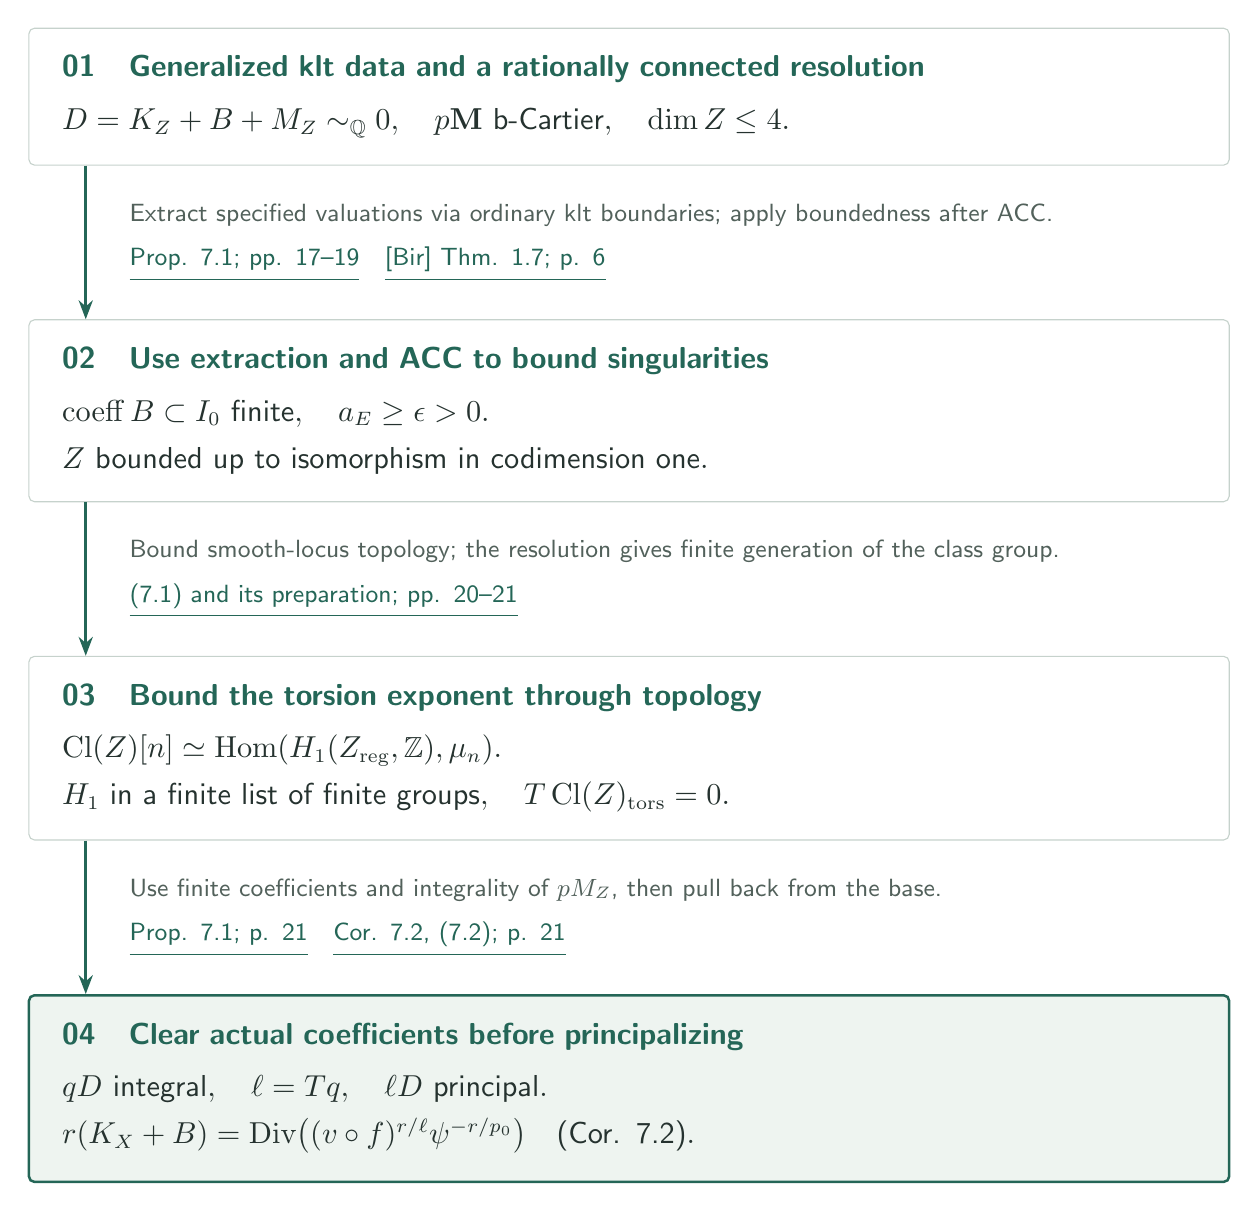
\begin{tikzpicture}
\node[card] (n0) {\heading{01}{一般化klt対と有理連結な解消}{Generalized klt data and a rationally connected resolution}$D=K_Z+B+M_Z\sim_{\mathbb Q}0,\quad p\mathbf M\text{ b-Cartier},\quad\dim Z\le4.$};
\node[card,below=1.95cm of n0] (n1) {\heading{02}{抽出とACCで特異点を一様にする}{Use extraction and ACC to bound singularities}$\operatorname{coeff}B\subset I_0\text{ finite},\quad a_E\ge\epsilon>0.$\\[3pt] $Z\text{ bounded up to isomorphism in codimension one}.$};
\flow{n0}{n1}{\Tx{通常のklt境界で指定付値を抽出。ACCの後に有界性を適用。}{Extract specified valuations via ordinary klt boundaries; apply boundedness after ACC.}\\[4pt]\Cite{https://github.com/openai/math/blob/adc7f1241b42e322a6451854ab7e4b4c146bf78a/preprints/Relative-denominators-and-effective-systems-for-log-Calabi-Yau-fibrations-September-27-2026/paper.pdf}{Prop. 7.1; pp. 17--19}\quad \Cite{https://arxiv.org/pdf/2305.18770v2}{[Bir] Thm. 1.7; p. 6}}
\node[card,below=1.95cm of n1] (n2) {\heading{03}{位相からtorsionの指数を抑える}{Bound the torsion exponent through topology}$\operatorname{Cl}(Z)[n]\simeq\operatorname{Hom}(H_1(Z_{\rm reg},\mathbb Z),\mu_n).$\\[3pt] $H_1\text{ in a finite list of finite groups},\quad T\operatorname{Cl}(Z)_{\rm tors}=0.$};
\flow{n1}{n2}{\Tx{有界な滑らかな開集合の位相と、解消からのclass group有限生成。}{Bound smooth-locus topology; the resolution gives finite generation of the class group.}\\[4pt]\Cite{https://github.com/openai/math/blob/adc7f1241b42e322a6451854ab7e4b4c146bf78a/preprints/Relative-denominators-and-effective-systems-for-log-Calabi-Yau-fibrations-September-27-2026/paper.pdf}{(7.1) and its preparation; pp. 20--21}}
\node[result,below=1.95cm of n2] (n3) {\heading{04}{実際の因子を整にして主因子化する}{Clear actual coefficients before principalizing}$qD\text{ integral},\quad \ell=Tq,\quad \ell D\text{ principal}.$\\[3pt] $r(K_X+B)=\operatorname{Div}\bigl((v\circ f)^{r/\ell}\psi^{-r/p_0}\bigr)\quad\text{(Cor. 7.2)}.$};
\flow{n2}{n3}{\Tx{有限係数集合と $pM_Z$ の整性を使い、底から引き戻す。}{Use finite coefficients and integrality of $pM_Z$, then pull back from the base.}\\[4pt]\Cite{https://github.com/openai/math/blob/adc7f1241b42e322a6451854ab7e4b4c146bf78a/preprints/Relative-denominators-and-effective-systems-for-log-Calabi-Yau-fibrations-September-27-2026/paper.pdf}{Prop. 7.1; p. 21}\quad \Cite{https://github.com/openai/math/blob/adc7f1241b42e322a6451854ab7e4b4c146bf78a/preprints/Relative-denominators-and-effective-systems-for-log-Calabi-Yau-fibrations-September-27-2026/paper.pdf}{Cor. 7.2, (7.2); p. 21}}
\end{tikzpicture}

\end{document}
